\section{Anhang}

Das folgende Lemma benötigen wir, um den Definitionsbereich einer Abbildung so \enquote{fein} aufteilen zu können, dass wir auf den Teilstücken lokale Inverse finden. Diese benutzen wir, um lokale Hochhebungen zu kontruieren.
\begin{convention}
	Ein Ball in einem metrischen Raum ist bei uns immer offen.
\end{convention}
\begin{lemma} [Lebesgue] \label{lemma_lebesgue_number}
	Sei \((K,d)\) ein kompakter, metrischer Raum und \(\mathcal{U}\) eine offene Überdeckung von \(K.\) 
	Dann gibt es ein \(\delta > 0\), sodass für alle \(x\in K\) ein \(U\in\mathcal{U}\) existiert, die den Ball \(B_{\delta} (x) \subseteq U\) vollständig enthält.

\iffalse
	Sei \(f:I^n \longarrow X\) eine stetige Abbildung in einen topologischen Raum \(X.\) Sei außerdem \(\mathcal{V}\) eine offene Überdeckung von \(X\). Dann gibt es ein \(N\in\N\), sodass für alle \(I_i:=[\frac{i-1}{N}, \frac{i}{N}]\) das Bild \(f(Q)\)eines Teilwürfels \(Q:=I_{i_1}\times \dots \times I_{i_n}\) vollständig in einer Menge \(V\in\mathcal{V}\) enthalten ist. Dabei sind \(i,i_1,\dots,i_n \in \{1,\dots, N\}\)
\fi
\end{lemma}
\begin{idea}
	\begin{wrapfigure}{r}{3cm}
		\setbox0\hbox{
			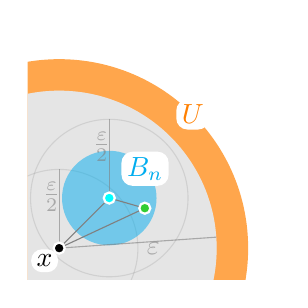
\begin{tikzpicture}[scale=2]
			\clip (-0.2,-0.2) rectangle (1.4,1.4);
			%U
			\fill[opacity=0.7, orange] (0,0) circle (1.2cm);
			\fill[white] (0,0) circle (1cm);
			%epsilon
			\begin{scope}[gray, opacity=0.2]
				%\fill[orange] (0,0) circle (1.3cm);
				%\fill[opacity=1, green!20!white] (0,0) circle (1cm);
				\fill (0,0) circle (1cm);
				\draw (0,0) circle (0.5cm);
				\draw (45:0.45cm) circle (0.5cm);
				\fill[cyan, opacity = 0.5] (45:0.45cm) circle (0.3cm);
			\end{scope}
			%epsilon Beschriftungen
			\begin{scope}[opacity=0.6, gray]
				\draw (0,0) -- 
					node[pos=0.6, below=-3pt] {$\varepsilon$} ++(4:1cm);
				\draw (45:0.45cm)
					-- node[pos=0.65, left=-4pt] {$\frac{\varepsilon}{2}$} 
					++(0,0.5cm);
				\draw (0,0)
					-- node[pos=0.65, left=-4pt] {$\frac{\varepsilon}{2}$} 
					++(0,0.5cm);
			\end{scope}
			%Dreieck
			\begin{scope}[opacity=1, gray]
				\draw (0,0) -- (45:0.45) -- (25:0.6cm) -- (0,0);
				
			\end{scope}
			%Punkte und Beschriftungen
			\begin{scope}[inner sep=2pt, fill=black, draw=white, thick]
				\filldraw (0,0) circle (1pt)
					node[fill=white, below left, rounded corners] {$\color{black}x$};
				\filldraw[fill=Cyan] (45:0.45cm) circle (1pt)
					%node[fill= white, below right, rounded corners] {$\color{cyan}x_n$}
					;
				\node at (45:0.5cm) [fill=white, rounded corners, inner sep = 2pt, above right=+2pt]  {$\color{cyan}B_n$};
				\filldraw[fill=LimeGreen] (25:0.6cm) circle (1pt);
				\node at (45:1.2cm) [rounded corners, fill=white, inner sep=2pt] {$\color{orange}U$};
			\end{scope}
			
		\end{tikzpicture}
		}
	\ht0=70pt
	\box0
	\end{wrapfigure}
	Wir nehmen an, dass die Behauptung falsch ist, sodass es eine Folge beliebig kleiner Bälle gibt, von denen aber keiner vollständig in einem \inlinebox{{$\color{orange}U$}}\(\in\mathcal{U}\) enthalten ist.
	Kompaktheit liefert uns einen Häufungspunkt \(\color{black} x\) dieser Bälle.
	Die Offenheit von \(U\) impliziert, dass es in der Nähe von \(x\) einen Ball \inlinebox{$\color{cyan}B_n$} geben müsste, der vollständig in \(U\) liegt\footnote{
		Die Skizze erläutert bereits die Beweisschritte unten. Wir verwenden die Dreiecksungleichung, um zu zeigen, dass ein beliebiger Punkt 
		\inlinebox{$\color{LimeGreen} y$}
		aus \(B_n\) innerhalb einer \(\varepsilon\)-Umgebung um \(x\) liegt.
	}; das widerspricht aber unserer Annahme.
\end{idea}
\begin{proof}
	Wir präzisieren die Beweisidee. Angenommen, für alle \(\delta> 0\) existiert ein \(x\in K\), sodass für alle \(U\in\mathcal{U}\) gilt, dass \(B_\delta (x)\nsubseteq U.\) Dann gibt es eine Folge \((x_n)_{n\in\N}\) in $K$, sodass für alle  \(U\in\mathcal{U}\) gilt: 
	\begin{equation} \label{lemma_lebesgue_proof_eq_notinU}
		B_n:=B_{\frac{1}{n}} (x_n)\nsubseteq U.
	\end{equation}
	Wir machen jetzt mehrere Beobachtungen:
	\begin{enumerate}
		\item Da die Überdeckung offen ist, gibt es für alle \(x\in K\) ein \(\varepsilon>0\), sodass \(B_\varepsilon (x) \subseteq U\) für ein \(U\in\mathcal{U}.\)
		\item Da \(\lim_{n\arrow 0} \frac{1}{n}=0\) ist, gibt es für alle \(\varepsilon>0\) ein \(N\in \N\), sodass für alle \(n\geq N\) gilt, dass \(B_n \subset B_\frac{\varepsilon}{2} (x_n)\).
		\item Da kompakte metrische Räume folgenkompakt sind, gibt es ein \(x\in K\),
		 sodass es für alle \(\varepsilon > 0\) unendlich viele \(n\in \N\) gibt, sodass \(x_n\in B_\frac{\varepsilon}{2} (x)\). Insbesondere gilt das für unendlich viele \(n\geq N\), wobei \(N\in\N\) beliebig.
	\end{enumerate}
	Lässt man sich von der Reihenfolge der Quantoren nicht verwirren, gibt es \(\epsilon>0\), \(U\in\mathcal{U}\), \(x\in U\) und \(n\in \N\), sodass
	\begin{center}
		\begin{enumerate*} [itemjoin={, \quad}] 
		\item \label{lemma_lebesgue_proof_item_ball_in_U}\(B_\varepsilon (x)\subset U\)
		\item \label{lemma_lebesgue_proof_item_Bn_in_eps_half}\(B_n\subseteq B_\frac{\varepsilon}{2}(x_n)\)
		\item \label{lemma_lebesgue_proof_item_xn_in_half_eps}\(x_n \in B_\frac{\varepsilon}{2} (x).\)
	\end{enumerate*}
	\end{center}
	
	\begin{claim}
		Es gilt \(B_n\subset B_\varepsilon (x).\)
	\end{claim}
	\begin{proofofclaim}
		Sei \(y\in B_n\). Die Dreiecksungleichung liefert zusammen mit \ref{lemma_lebesgue_proof_item_Bn_in_eps_half} bzw. \ref{lemma_lebesgue_proof_item_xn_in_half_eps}:
		\[d(y,x)\leq d(y,x_n) + d(x_n,x)< \frac{\varepsilon}{2}+\frac{\varepsilon}{2} = \varepsilon.\]
	\end{proofofclaim}

	Damit erhalten wir wegen \ref{lemma_lebesgue_proof_item_ball_in_U} einen Widerspruch zu \cref{lemma_lebesgue_proof_eq_notinU}, denn es müsste gelten:
	\[B_n\subset B_\varepsilon (x)\subseteq U. \quad\text{\lightning}\]

\iffalse
	Da \(I^n\) kompakt ist, gibt es ein Teilsystem \(\mathcal{V}'\subset \mathcal{V}\), sodass
		\[\mathcal{U}:= \{f^{-1}(V)\mid V \in \mathcal{V}' \}\] 
	eine endliche Überdeckung von \(I^n\) ist. Angenommen, für alle \(N\in\N\) gibt es einen Teilwürfel \(Q_N\), sodass \(Q\nsubseteq U\) für alle \(U\in\mathcal{U}\) ist. Da die Mengen \(U\) offen sind, gibt es für jeden Punkt \(t\in I^n\) eine offene Umgebung, die vollständig in \(U\) enthalten ist. Da \(\mathcal{U}\) endlich ist
\fi
\end{proof}



\begin{proof}
Sei \(V\subset Y\) offen. Dann ist
\[f^{-1} (V) = f^{-1} ( V) \cap X
=  f^{-1} (V) \cap \bigcup_{U\in \mathcal{U}} U 
= \bigcup_{U\in \mathcal{U}} f^{-1}(V) \cap U
= \bigcup_{U\in \mathcal{U}} f_{|U}^{-1}(V)
\]
als Vereinigung offener Mengen offen. Der Beweis für endlich viele abgeschlossene Mengen verläuft analog.
\end{proof}

\begin{lemma}[Das Eckige muss ins Runde] \label{lemma_hypercube} 
	Ein Hyperwürfel \(Q\subset\R^n\) mit Kantenlänge \(a\) liegt vollständig in einem Ball mit Radius \(a\sqrt{n}\). 
\end{lemma}
\begin{proof}
	Da Translation längenerhaltend ist, können wir ohne Einschränkung annehmen, dass der Mittelpunkt des Würfels am Ursprung liegt. Das heißt
	\(Q=\prod_{i=1}^n\big[-\frac{a}{2},+\frac{a}{2}\big]\).
	Für alle \(x\in Q\) ist also \(x_i^2 \leq \frac{a^2}{4}\) und somit
	\(\Norm{x}= \sqrt{x_1^2 + \dots + x_n^2} \leq \sqrt{n\cdot \frac{a^2}{4}} = \frac{a}{2}\sqrt{n} < a\sqrt{n}.\)
\end{proof}
\begin{corollary_weak} [Lebesgue-Anwendung]
	Sei \(f:I^n \longarrow X\) eine stetige Abbildung in einen topologischen Raum \(X\) und \(\mathcal{V}\) eine offene Überdeckung von \(X\). Dann gibt es ein 
	\(N\in\N\), sodass für alle 
	\(I_i:=[\frac{i-1}{N}, \frac{i}{N}]\) das Bild \(f(Q)\)eines Teilwürfels \(Q:=I_{i_1}\times \dots \times I_{i_n}\) vollständig in einer Menge \(V\in\mathcal{V}\) enthalten ist. Dabei sind \(i,i_1,\dots,i_n \in \{1,\dots, N\}\)
\end{corollary_weak}
\begin{proof}
	\(I^n\) wird von \(\mathcal{U}:=\{f^{-1}(V)\mid V\in\mathcal{V}\}\) überdeckt. 
	\cref{lemma_hypercube} liefert uns, dass jeder Teilwürfel \(Q\) in einem Ball mit Radius \(\frac{\sqrt{n}}{2N}\) enthalten ist. Falls wir \(N\) groß genug wählen, liefert uns \cref{lemma_lebesgue_number}, dass \(Q\subset U\) für ein \(U\in\mathcal{U}\) und damit \(f(Q)\subset f(U)\in\mathcal{V}.\)
\end{proof}

\begin{lemma} [Verklebung] \label{lemma_pasting}
Sei \(f:X\longarrow Y\) eine Abbildung topologischer Räume und \(\mathcal{U}\) eine offene Überdeckung von \(X\), sodass für alle \(U \in \mathcal{U}\) die Einschränkung \(f_{|U}\) stetig ist. Dann ist auch \(f\) stetig. Das gleiche gilt, falls \(\mathcal{U}\) \emph{endlich} ist und nur abgeschlossene Mengen enthält.
\end{lemma}






\pagebreak
\nocite{*}
\printbibliography
